\section{Image Annotation}
The image annotation feature of this program uses a set of vertices to form a polygon; this polygon is used to highlight the desired object and distinguish it from the rest of the image. The user begins by clicking on the "Add" button and then on the screen at the desired locations to form the polygon. When all vertices have been placed the user finishes by either right-clicking on the picture or clicking on the "Add" button again.  Once the polygon has been drawn a window will pop up and ask for the name of the highlighted object, This dialogue is a modal window provided by the framework and is a standard way of getting small inputs. The name of the annotation is then displayed as a tool-tip whenever the user hovers over the polygon\ref{fig:fullView}.

There are several remarks that can be made about this feature. One problem that we had to deal with when we were implementing it was that a user may not necessarily select the vertices of the polygon in order. This situation is not supported by the underlying framework and produces undefined shapes. Our solution to this problem was to colour the surface of the polygon as the user adds the vertices. This results in a shape that is more intuitive for the user to visualise as they are drawing, and in this way guides them through the polygon creation and hence helps prevent erroneous shapes.

\begin{figure}[h!]
\centering
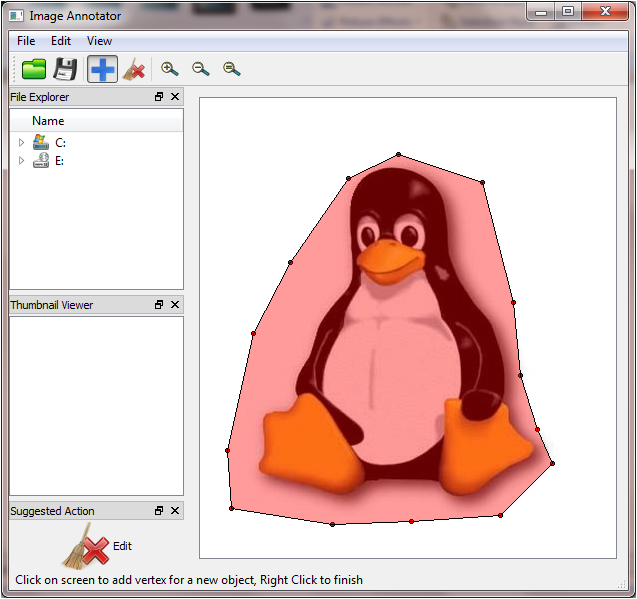
\includegraphics[width=6cm]{example.png}
\caption{Main Window of the application with an example of an annotated object}
\label{fig:fullView}
\end{figure}

Another design decision we made when implementing the drawing feature was to not include the ability for the user to edit the position of each vertex of the polygon once it had been created. This means that after the user names the polygon it can no longer change shape - it must be deleted and redrawn. This decision was primarily based on time constraints since we had other features that we felt were a greater priority.  However, in defense of our decision annotations are usually small and therefore a user may prefer to redraw the polygon anyway, rather than changing and/or adding extra vertices as this may take longer to accomplish.
